TODO

\section{Technology}
In this section, technologies used in the transformation program that will be mentioned throughout this chapter are briefly described.

\subsection{Django}
Django is a Python web development framework \cite{holovaty_chapter_c1itd}. It implements a version of the MVC (Model-View-Controller) pattern, which decouples request routing, data access, and
presentation. Django's model layer allows the programmer to retrieve and modify entities in an SQL database through Python code, without writing SQL.

\subsection{MySQL}
MySQL is an open source relational database system \cite{what_wim}. It is used by TriOptima as the database backend for Django.

\subsection{Cassandra}
Cassandra is a column-oriented \textit{NoSQL} database \cite[p. 1-9]{mishra_2014_beginning_bacd}. It features dynamic schemas, meaning that columns can be added dynamically to a schema as needed, and that
the number of columns may vary from row to row. Cassandra is designed to have no single point of failure, and uses a number of nodes in a peer-to-peer structure. This design is
employed in order to ensure high availability, with data replicated across the nodes.

\section{Performance analysis tools}
\subsection{cProfile}
A Python profiler with a relatively low overhead, which can be invoked both directly in a Python program and form the command line \cite{26_2tppp2d}.

\subsection{resource}
\code{resource} is a Python module used for measuring resources used by a Python program \cite{36_3rruip2d}. It can be used for finding the user time, system time,
and the maximum memory used by the process.

\section{Trade files and datasets}
As mentioned briefly in section \ref{trioptima}, users of the triResolve service upload \textit{trade files}, which contain one or several datasets with
rows of trade data such as party id, counterparty id, trade id, notional, and so on. An example of a trade dataset (with some columns omitted) can be seen in figure
\ref{fig:data_set_example}.

\begin{figure}[ht]
\centering
\resizebox{\linewidth}{!}{%
\begin{tabular}{|c|c|c|p{3cm}|c|c|}%
  \hline
  \bfseries Party ID & \bfseries CP ID & \bfseries Trade ID & \bfseries Product class & \bfseries Trade curr & \bfseries Notional
  \csvreader[respect all,head to column names]{figures/EFET.csv}{PARTY_ID=\pid, CP_ID=\cpid, TRADE_ID=\tid, PRODUCT_CLASS=\pcls, TRADE_CURR=\tc, NOTIONAL=\notional}
  {\\\hline \pid & \cpid & \tid & \pcls & \tc & \notional}
  \\ \hline
\end{tabular}}
  %\centering
\caption[Example of trade dataset]{A simplified example of a trade dataset uploaded by the users of triResolve.}
  \label{fig:data_set_example}
\end{figure}

\section{File formats}
Different customers may have different ways of formatting their datasets, with different names for headers, varying column orders, extra fields,
and special rules. In order to convert these into a standard format that make it possible to use the files in the same contexts, a file format specifying
how the dataset in question should be processed is used. The format contains a set of \textit{filters} which should be applied to each row of the dataset.
The different filter configurations may affect how parallelizable the processing of the dataset is.

\section{Verification results}
The result of the dataset processing is called a \textit{verification result}\footnote{The verification results are not to be confused with the results of this thesis. They are part of the problem this thesis aims to solve.}, and consists of one row per trade, with correctly modified values, in a Cassandra schema.
In addition, a row in the MySQL database consisting of metadata relating to the result as a whole is created. This metadata includes result owner, number of rows, time metrics, and so on.

\section{Transformation with constraints}
\subsection{Filters}
All filters used to transform a dataset into a verification result are outlined below.

\begin{itemize}
\item \textbf{Header detection} --
There may be a number of initial lines in the dataset which do not contain the header (which specifies the column names). The header detection filter checks if a row is the header,
and if it is it saves the column names and corresponding indices for use in subsequent rows. If the row is not the header or the header has already been detected
(for example if another header row is encountered in the middle of the dataset), this filter terminates without any effect and the rest of the filters are applied.
This filter is included in all file formats.

\item \textbf{Mapping} --
Maps a value from a column in the dataset to a specified output column in the verification result. There is usually a mapping for each of the columns in the input
dataset, and the Mapping filter is therefore one of the most common filters. The mappings may have small extra tuning attached to them, such as specifying a date
format or extracting only part of the text using regex. One of these extra tunings is attached to the trade id column, and is called \textit{Make unique}.
This tuning keeps track of all trade id:s that have been encountered so far, and, if it finds a duplicate, adds a suffix to it in order to ensure that all trade id:s are unique.

\item \textbf{Dataset translation} --
A dataset translation is similar to a mapping, but uses specified columns in an external dataset to map input columns to output columns.

\item \textbf{Dataset information} --
Extracts information about the dataset, such as the name or owner.

\item \textbf{Tradefile information} --
Similar to the dataset information filter, except that it extracts information about the trade file that contains the dataset.

\item \textbf{Null translation} --
In some datasets, other values than \code{NULL} are used to convey the absence of a value. This filter allows the user to specify which other values
should be interpreted as \code{NULL}.

\item \textbf{Relation currency} --
If the currency that is supposed to be used in a relation (a party and a counterparty) is stored in the database and should be mapped to an output column, this
filter retrieves this information.

\item \textbf{Global variable} --
A global variable filter writes a value to a variable that is accessible by subsequent filters on the same row, and by all filters on the rest of the rows in the data
set. A global variable can be written several times throughout the processing of a dataset.

\item \textbf{State variable} --
A state variable is similar to a global variable, but is always written to before all other processing of the dataset begins.

\item \textbf{Temporary variable} --
Similar to the other variables, except for the fact that it is only accessible during processing of the row where it was written. When the 
processing of the row is finished, the variable is cleared.

\item \textbf{Conditional block} --
A conditional block works like the programming construct \code{if}. It performs a specified filter (which may also be a conditional block) only if a certain
condition is fulfilled. Most commonly, the condition takes the form '\code{field = value}', but may also involve more complex expressions in the form of a
subset of Python.

\item \textbf{Logger} --
A logger filter simply logs a given value. Can for instance be used when a user wants to know whenever a conditional block has been entered.

\item \textbf{Skip row} --
Ignores the current row when processing. Usually used in a conditional block.

\item \textbf{Stop processing} --
Stops processing the dataset, ignoring all subsequent rows. Can be used as a subfilter in the Conditional block filter when the footer of the dataset
contains information that should not be interpreted as a trade.

\item \textbf{Third party automapper} --
When a customer has uploaded a trade file on behalf of another customer, this filter extracts the information needed to make sure that the data is loaded
for the correct customer.

\item \textbf{Set value} --
Simply sets the value of the output column to the value that is entered.

\item \textbf{RegExp extract} --
Extracts text from a column using regex, and writes matching groups to other columns.

\item \textbf{RegExp replace} --
Replaces column text matching some regex with a specified value.

\end{itemize}

An example of how filter application and dataset row transformation work can be found in figure \ref{fig:filter_diagram}.

\begin{figure}[ht]
  \centering
  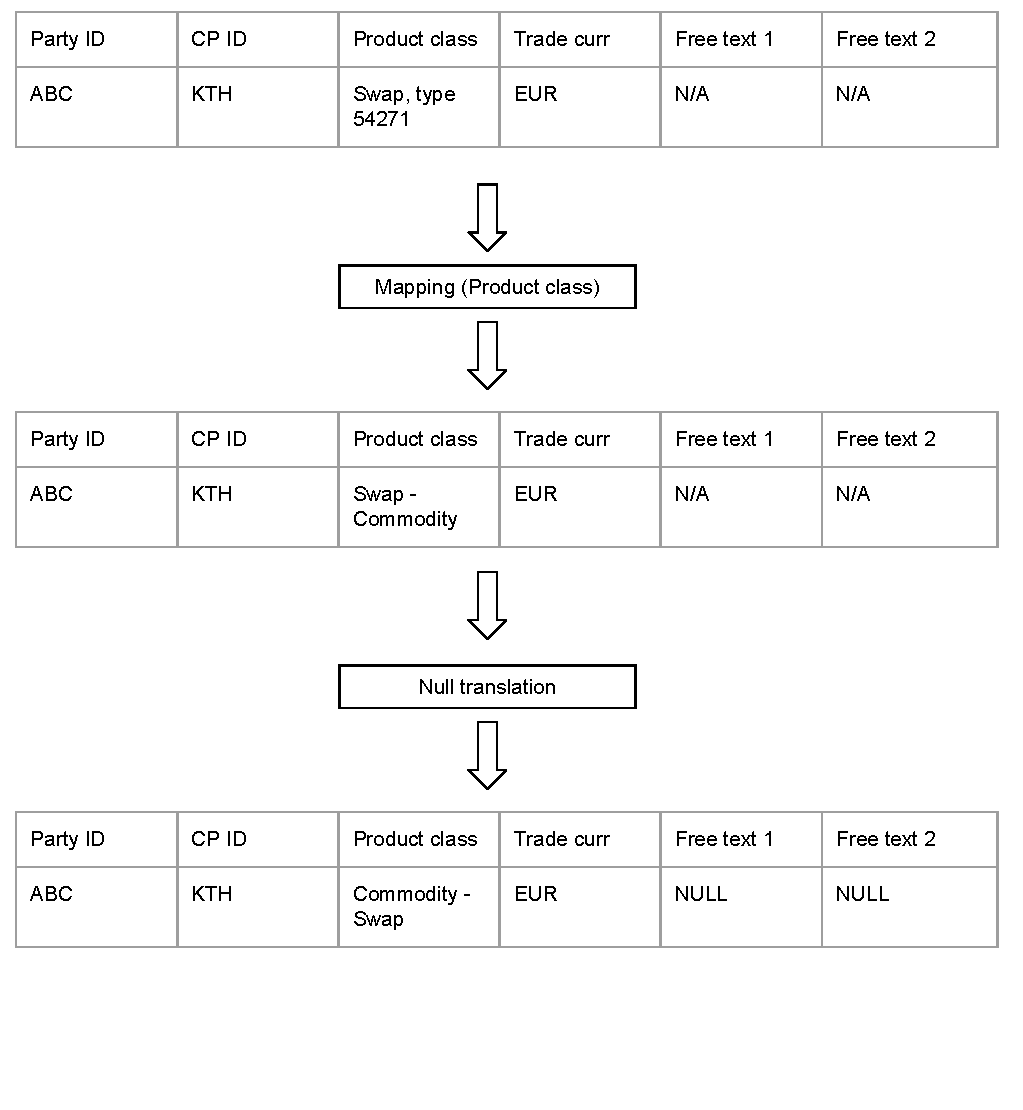
\includegraphics[width=120mm]{figures/filter_diagram.pdf}
  \caption[Filter application example.]{A simplified example of how filter application and dataset transformation work. The mapping filter for the
  product class column is applied, transforming ``Swap, type 54271'' to the standardized ``Swap - Commodity ''. In the file format used for this example,
  ``N/A'' is used to denote the absence of a value, making the null translation filter translate all columns containing ``N/A'' to ``NULL''.}
  \label{fig:filter_diagram}
\end{figure}

\section{Program overview}
The general flow of the original, sequential, dataset processing program is the following:
\\\\
The unprocessed dataset has the rows stored in a Cassandra database, and some metadata and methods stored in a Django object backed by a MySQL database.
The file format corresponding to the dataset is looked up, and all of the filters it contains are added to a pipeline that will process the dataset.
An empty verification result is then created in both Cassandra and MySQL, containing the row data and result metadata with metrics, respectively.
The metrics include processing time, number of trades, timestamp, and similar data. The rows in the dataset are then processed one by one,
applying all filters to each row. As soon as a row has finished processing, it is written to the verification result in Cassandra.
During this process, the row mappings used in the \textit{Mapping} filter are fetched from the MySQL database, resulting in some
I/O waiting time. To mitigate this, the mappings are cached in memory for faster access. After the processing has finished, the result metadata
and metrics are saved in the MySQL database.

A simplified overview of the sequential program can be found in figure \ref{fig:sequential_program_overview}.

\begin{figure}[ht]
  \centering
  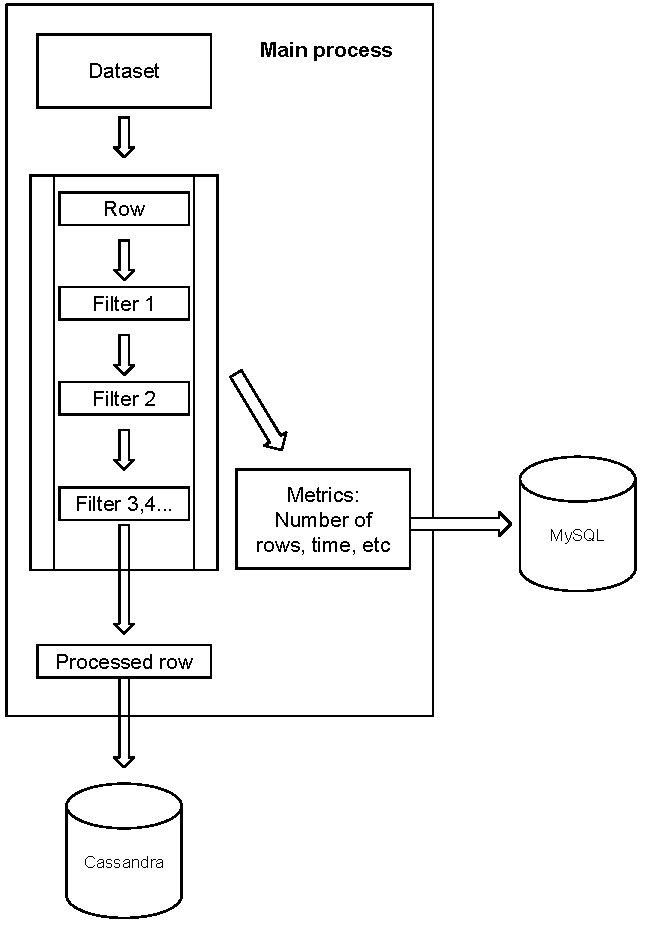
\includegraphics[width=120mm]{figures/program_overview_sequential.pdf}
  \caption[Sequential program overview.]{Sequential program overview.}
  \label{fig:sequential_program_overview}
\end{figure}

\section{Sequential program profiler analysis} \label{section:sequential_profiler}
The result of running \code{cProfile} on the sequential transformation program can be found in figure \ref{fig:sequential_profiler}. The dataset used had
27877 rows, 46 columns, and belonged to the extra overhead file format family.
Function calls with very low cumulative time have been omitted. In the profiling result, \code{ncalls} is the number of times the function was called,
\code{tottime} is total time spent in the function (excluding subfunctions), \code{cumtime} is the total time spent in the function
including its subfunctions, and \code{percall} is the quotient of \code{cumtime} divided by primitive calls \cite{26_2tppp2d}.

\begin{figure}[ht]
  \lstinputlisting[basicstyle=\tiny]{figures/profiling_17_may_short.txt}
  \caption{Sequential program \code{cProfile} output}
  \label{fig:sequential_profiler}
\end{figure}

From the profiling information above, it is clear that some function calls take significantly more time than others, and are therefore
interesting targets for parallelization analysis. The \code{process} method is the one that launches the main pipeline that applies all
filters and performs the transformation of the dataset. The fact that it takes 66.280 seconds out of 66.567 is therefore expected. Among
the functions that \code{process} calls, \code{process\_record}, \code{post\_process\_record}, \code{consume\_record}, and \code{\_prepare} are the most
interesting. Other functions with relatively high cumulative time are called from these functions.
\begin{itemize}
  \item \code{process\_record} -- In the profiling information, \code{process\_record} appears twice, once in the file \code{pipeline.py} and once in the file
    \code{mappings.py}. The version in \code{pipeline.py} is abstract, with an implementation in each of the filters. It is evident that the implementation
    that is most common resides in \code{mappings.py} as it is the only one that shows up among the function calls that take up a significant amount of time.
    This is expected, as \textit{Mapping} is the most common filter and represented in \code{mappings.py}. The function has a low \code{percall} and a high
    \code{ncalls}, indicating that the reason it takes up a large portion of the total time is the fact that it is called many times due to the many filters
    and dataset rows. \code{process\_record} takes up 35.0\% of the total execution time.
  \item \code{post\_process\_record} -- Similarly to \code{process\_record}, \code{post\_process\_record} is an abstract method and is implemented in all filters.
    It also has a low \code{percall} and a high \code{ncalls}. \code{post\_process\_record} takes up 33.1\% of the total time.
  \item \code{consume\_record} -- This method calls \code{\_write\_record}, which is the method that writes rows to Cassandra after they have been transformed.
    \code{consume\_record} is called once per row and takes 8.4\% of the total time, and \code{\_write\_record} is responsible for 7.9\% of these. 
  \item \code{\_prepare} -- Called once before the program starts iterating over all rows, performing setup needed to perform the transformations properly.
    It has a relatively high \code{percall} and takes up 3.3\% of the total execution time.
\end{itemize}
The time spent in the functions above is 87.7\% of the toal time, and the majority of the rest of the code in \code{process} is contained in the body of the loop that iterates
over and performs actions on every row. Since only \code{\_prepare} runs before the loop, and a small portion of code is run after the loop, about 4\% of the code 
is run outside the loop. This means that around 96\% of the code is conceivably parallelizable, depending on the filters in the dataset's file format.\\

The following conclusions can be made from the analysis above:

\begin{itemize}
  \item A majority of the functions responsible for most of the time consumption have low \code{percall} and high \code{ncalls}, indicating that no single function is
    a significant bottleneck, and that the major reason these functions take up large portions of the total time is that they are called a high number of times.
  \item A relatively small portion of the code is spent in functions that perform I/O, indicating that the program is CPU bound and suitable for speedup using
    \code{multiprocessing}.
  \item Close to all of the code in \code{process} is run for each row, indicating that performing the transformation of different rows in different tasks is a
    suitable granularity when implementing the parallelization.
  \item The fact that \code{\_prepare} takes up a non-negligible part of the program and is called before the processing of each row, it may introduce extra overhead
    when parallelizing, since it may need to be called for each worker.
\end{itemize}

\section{Performance model calculations}
In this section, different performance calculation models are used to find a preliminary indication of possible speedup.

\subsection{Amdahl's law}
In the sequential profiling session, it is suggested that around 96\% of the code is parallelizable. The computer used for testing has 8 cores,
which is the value that will be used for the $n$ value when applying Amdahl's law to the profiling session run:

\begin{displaymath}
  S = \frac{1}{1 - 0.96 + \frac{0.96}{8}} = 6.25
  \label{fig:amdahl_calculation}
\end{displaymath}

\noindent This potential speedup of 6.25 does not take into account overhead associated with parallelization.

\subsection{Gustafson's law}
With Gustafson's law, the speedup is calculated as the following:

\begin{displaymath}
  S = 8 + (1-8) * 0.04 = 7.72
\end{displaymath}

\noindent With the more optimistic Gustafson's law, the speedup is higher. Overhead is not taken into account in the above calculation.

\subsection{Work-span model}
As mentioned in section \ref{work-span}, the increase in work when parallelizing a program should be kept to a minimum.
In addition, the span should be kept as small as possible. In the implementation made in this thesis, both the work and the span is increased.
The work is increased since the code that is run before the loop over each row has to be run once for each worker, and because the caching of
column mappings is done for each worker. The span is increased because of the added post processing needed when transforming datasets from the
extra overhead file format family. This suggests that parallelization cannot be utilized at its fullest, which may impact the speedup.

\section{Analysis of filter parallelizability}
Since the filters specify what the processing program should do to each row in a dataset, ``row by row'' or possibly chunks of rows is a suitable
granularity when implementing the parallelization of the program. Consequently, the filters of a file format are the prime candidates
for parallelization analysis. The analysis made is similar to the methodology used to identify the span in the work-span model described in
section \ref{work-span}. When applying the model to the problem of analyzing filters, a task is the processing of one row. In order to find
the tasks that need to be completed before other tasks, the filters that result in state that is accessed by subsequent rows or otherwise
affect the total processing of the dataset need to be identified.

Examining the filters, it is apparent that \textit{Dataset translation}, \textit{Null translation}, \textit{Relation currency},
\textit{Third party automapper}, \textit{Set value}, \textit{RegExp extract}, and \textit{RegExp replace} only operate on the current dataset row, with no side effects.
This means that they produce no state changes that affect subsequent rows, which means that they do not affect the parallelizability of a dataset.

Additionally, \textit{Dataset information}, \textit{Tradefile information}, \textit{Temporary variable}, \textit{Logger}, and \textit{Skip row} perform
operations that either pull information from resources that are available to all rows, or produce an effect that does not affect any other rows.
The \textit{Conditional block} filter only produces effects according to its subfilters (a set of the filters already mentioned), and does not affect parallelization by itself.
\\\\
Hence, the filters that can affect the parallelization of a dataset are:
\begin{itemize}
  \item \textit{Mapping}, since the trade id mapping may need to keep track of state that can be accessed in subsequent rows in order to make all id:s unique.
  \item \textit{Header detection}, since all rows beneath the (first) header row depend on the column names for mappings and other values.
  \item \textit{Global variable}, since the variable may be written and accessed by any subsequent rows. Each rewrite of the variable needs to happen before the next rewrite,
    in the original, sequential order if the verification result is to be correct.
  \item \textit{State variable}, for the same reasons as Global variable.
  \item \textit{Stop processing}, if one thread sees a conditional fulfilled and stops processing, it is possible for another thread to keep processing rows that are intended
    to be ignored, thereby violating the constraints.
\end{itemize}

\section{Code inspection}
After an initial code and file format inspection, the following conclusions where made:
\begin{itemize}
  \item The \textit{Header detection} filter is effectively performed only once, as it is ignored for all rows after the one where the header was found.
  \item The filters \textit{Global variable} and \textit{State variable} make the processing of every row depend on the previous, as the writing of the variables may happen on each row.
  \item The process of making an ID unique could possibly be broken out to a post processing step.
  \item All file formats contain \textit{Header detection}, and many contain the make unique feature of the trade ID mapping.
  \item There are many file formats that do not have either \textit{Global variable}, \textit{State variable} or \textit{Stop processing} among their filters.
\end{itemize}

The conclusions above indicate that header detection may be done before creating the parallel processes, sending this data to each process when they are created.
If the process of producing unique ID:s is then done as a post processing step, the following task DAGs illustrate how the dependencies when processing different
file formats appear: In figure \ref{fig:embarrassing_dag}, the task DAG for a file format without a Global variable or State variable filter is illustrated.
In figure \ref{fig:embarrassing_dag}, the task DAG for a file format containing a Global variable is illustrated. Since the span is equal to the work
in the file formats containing Global variables or State variables, parallelization of datasets with these formats will result in no speedup according to the %Illustrate work-span?
work-span model (as $T_1 \leq T_\infty \Rightarrow S \leq 1$). File formats containing \textit{Stop processing} make it unfeasible to produce correct verification results
when parallelizing. Determination of whether the result is correct is non-viable if any rows are processed in different processes (as rows that should not be included in the result may be included anyway).

\begin{sidewaysfigure}[ht]
  \centering
  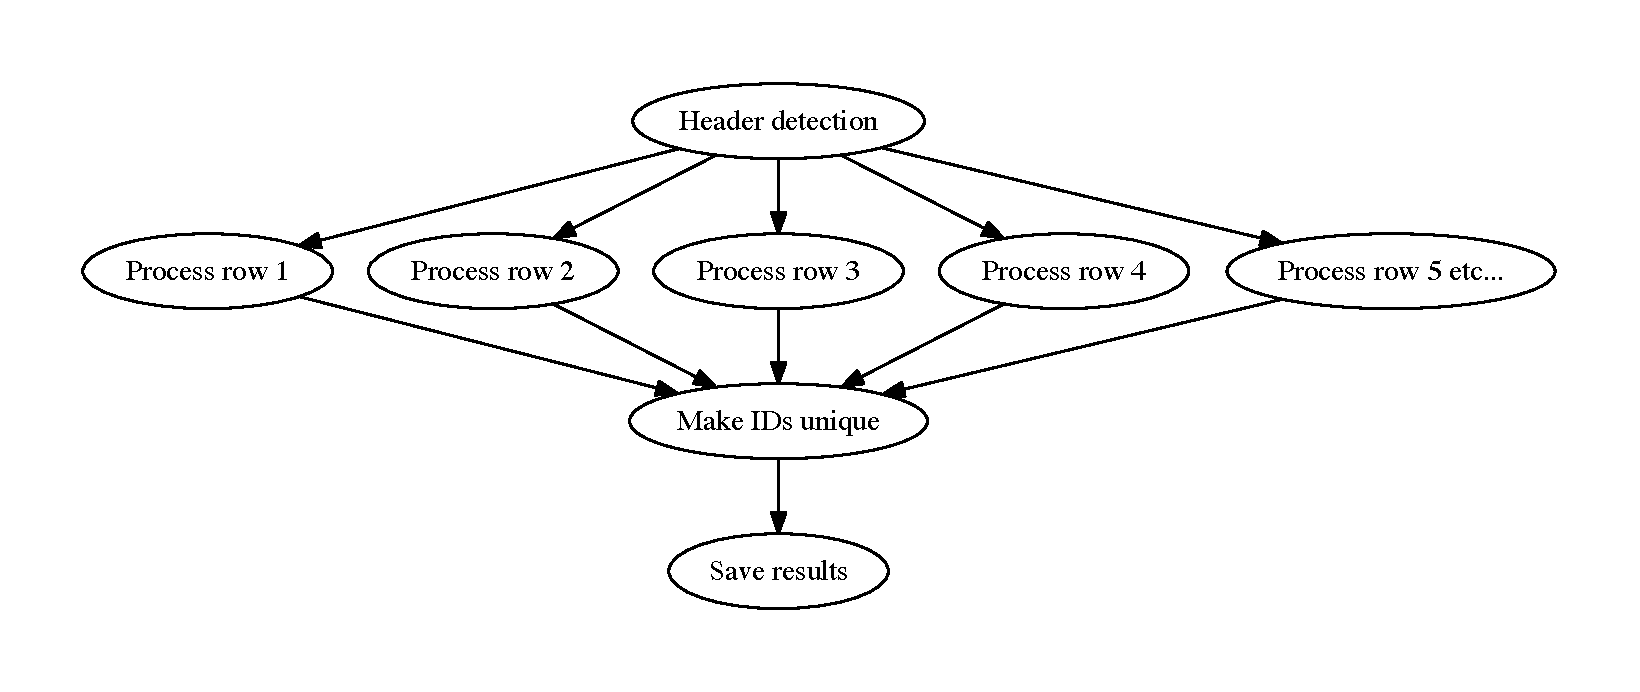
\includegraphics[width=200mm]{figures/embarrassing_file_format.pdf}
  \caption[Task DAG for a file format that does not contain global or state variables.]{An example of a task DAG for a file format that does not contain global variable or state variables. Header detections needs
  to be performed up front, and making trade IDs unique needs to be performed in a post processing step. The processing of each row does not depend on each other.}
  \label{fig:embarrassing_dag}
\end{sidewaysfigure}

\begin{figure}[ht]
  \centering
  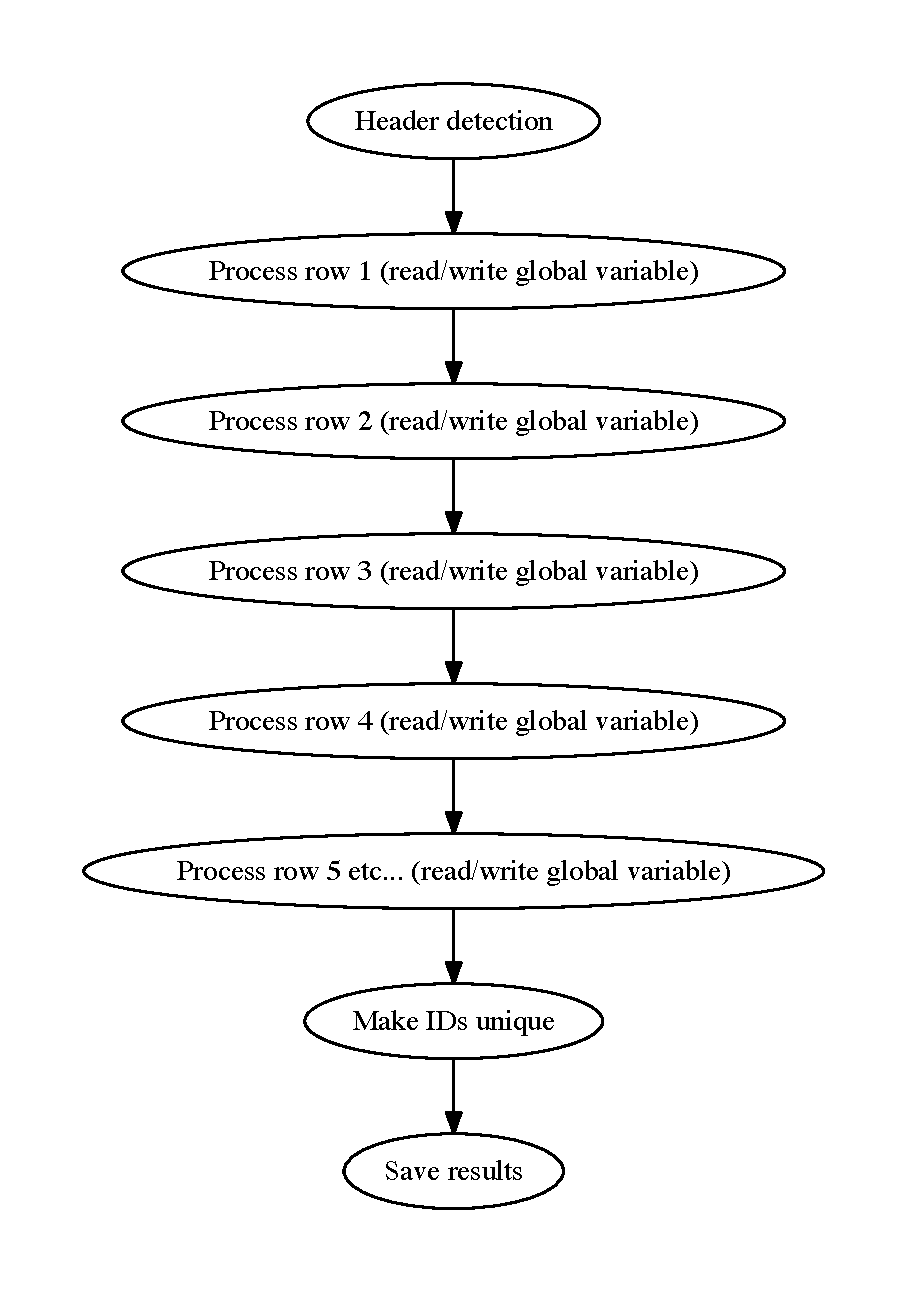
\includegraphics[width=120mm]{figures/global_variable_file_format.pdf}
  \caption[Task DAG for a file format that contains global or state variables.]{An example of a task DAG for a file format that contains global or state variables. Since each row may read and
  write the global (or state) variable, every task depends on the previous task.}
  \label{fig:global_dag}
\end{figure}

\section{Filter families}
With the help of the findings from the previous sections, families of filters with different characteristics can be identified.

\begin{itemize}
\item \textbf{Embarrassingly parallel filters} --
The filters that do not affect parallelization in any way are:
\textit{Dataset translation}, \textit{Null translation}, \textit{Relation currency},
\textit{Third party automapper}, \textit{Set value}, \textit{RegExp extract}, \textit{RegExp replace},
\textit{Dataset information}, \textit{Tradefile information}, \textit{Temporary variable}, \textit{Logger}, \textit{Skip row}, and \textit{Conditional block}.
In addition, \textit{Mapping} is included among these filters if the make unique feature is disabled.
\item \textbf{Overhead filters} -- 
Filters that introduce parallelization overhead are: \textit{Mapping} (if the make unique feature is enabled) and \textit{Header detection}.
\item \textbf{Inherently serial filters} --
The filters that enforce serial execution of the entire transformation are: \textit{Global variable}, \textit{State variable}, and \textit{Stop processing}.
\end{itemize}

\section{File format families}
In addition to the filter families, the fact that the \textit{Header detection} filter is present in all file formats makes it possible to identify the following
file format families relevant to this thesis:

\begin{itemize}
\item \textbf{Embarrassingly parallel file formats} --
  File formats that with the exception of \textit{Header detection} contain only embarrassingly parallel filters. 
\item \textbf{Extra overhead file formats} --
  Formats that in addition to \textit{Header detection} and a number of embarrassingly parallel filters also contain \textit{Mapping} with the make unique filter enabled.
\item \textbf{Inherently serial file formats} --
  Formats that contain any of the inherently serial filters.
\end{itemize}

\section{Parallelization}
In accordance with section \ref{related_work}, the Python \code{multiprocessing} module was used to implement the parallelization of the program. Additionally, measures where taken to send as little
data as possible between processes and to avoid introducing excessive complexity to the codebase. The \code{multiprocessing.Queue} facility was chosen for communication between processes due to its
noted performance and built-in synchronization \cite{singh_2013_parallel_padpwprfmm}.

Before deciding to use the parallelized version of program, the list of filters in a file format is examined for any of the inherently serial filters
\textit{Global variable}, \textit{State variable}, or \textit{Stop processing}. If any of these are found, the
program falls back to its sequential version. Otherwise, the program carries on in accordance with figure \ref{fig:embarrassing_dag}. First, before creating any additional processes, the Header detection filter
is applied row by row until it produces a result (commonly after a few rows). Next, a (tunable) number of processes, as well as two queues are created. A number of row spans, or chunks, are then created by splitting
the rows beneath the header row into equally sized partitions. The first queue is used to transfer the data needed to process a chunk of the dataset, including the header data, the row span, and the result metadata.
In order to avoid errors and sending large objects between processes, only the primary key used to retrieve the result metadata object from the MySQL database is sent to the processes.
After this, the processes can independently retrieve the data. The second queue is used for sending the partial metrics objects for each chunk, and for indicating if a process is done processing
its data or if it encountered an error. Since all other results are written to the Cassandra database, this is the only information that needs to be sent to the main process. The queues can be
denoted the 'chunk queue' and the 'message queue', respectively.

In each of the created processes, the rows in the chunk are retrieved from the Cassandra database and a new object containing metrics for the chunk is created. The chunk is then processed as in the sequential program,
applying all filters to each row. The metrics object is updated during the processing, as in the original program. If the chunk was processed correctly, the metrics object is put on the message queue. Otherwise,
if an exception occurs, an error message is put on the queue instead. When all data in a process has finished processing, a message indicating that the process has finished its work is put on the message queue.

The main process continuously polls the message queue, and merges the partial metrics objects as they are polled from the queue. If an error message is encountered, an exception is raised on the main thread, mimicking the
behavior of the original sequential program. It also increments a counter whenever a done message is received from a process. When the counter is equal to the number of subprocesses, the main process stops waiting
for messages, and progresses with the post processing step of making the trade ID:s unique. Finally, the main process saves the result object with the corresponding merged metrics to the MySQL database. At this point,
the program has produced a finished verification result.

A simplified overview of the parallel program can be found in figure \ref{fig:parallel_program_overview}.

\begin{sidewaysfigure}[ht]
  \centering
  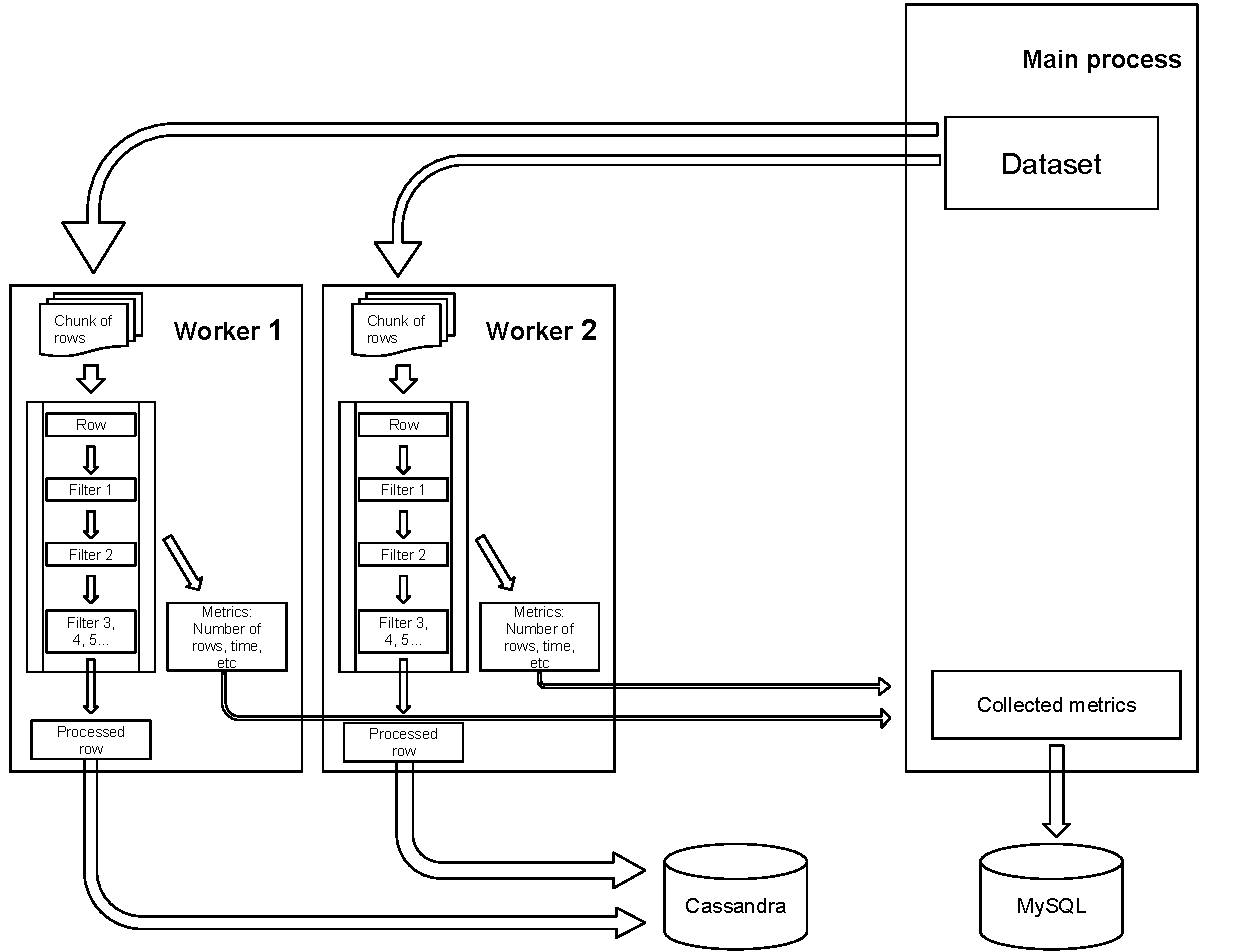
\includegraphics[width=200mm]{figures/program_overview.pdf}
  \caption[Parallel program overview.]{Parallel program overview.}
  \label{fig:parallel_program_overview}
\end{sidewaysfigure}

\section{Sources of overhead}
During the implementation of the parallel version of the program, the following possible sources of parallelization overhead where identified:

\begin{itemize}
  \item The \code{multiprocessing} module, where creating processes and transferring data between processes is costly.
  \item Less effective caching of mappings. Since the mappings cache is local to each subprocess, caches are built up individually. This results in fewer cache hits than in the sequential program, and more total work
    looking up values in the MySQL database. Hardware cache may also be affected in a similar manner.
  \item The process of making trade ID:s unique is added as an extra step after the main data processing pipeline.
  \item Because they lack built-in support for multiprocessing, the Python connections between both MySQL and Cassandra need to be restarted in the startup of each subprocess.
  \item \code{\_prepare} has to be called once for each of the workers, compared to only one call for the sequential program.
\end{itemize}

